\mode*
\section[Objetivos]{Objetivo general y objetivos espec\'ificos}
\label{sec:objs}

\mode<presentation>{
  \begin{frame}
    \transduration{1}
    \frametitle{Qu\'e se busca con esta investigaci\'on?}
    \begin{center}
      \LARGE \textbf{\textcolor{blueun}{Objetivo General y Objetivos Espec\'ificos}}
    \end{center}  
  \end{frame}
}
\subsection[General]{Objetivo general}
\label{sec:objgen}
\mode<presentation>{
  \begin{frame}[label=def_objetivos]
    \transduration<1->{5}
    \frametitle{Qu\'e se busca con esta investigaci\'on?}
    \textbf{\textcolor{blueun}{OG:}} Desarrollar un \alert<2>{marco de experiementaci\'on}\only<2-2>{\footnote{Marco o framework de investigaci\'on}}, mediante el cual se pueda implementar las hip\'otesis de soluci\'on de \alert<3>{los problemas de locomoci\'on}\only<3-3>{\footnote{Problemas actuales de robotica b\'ipeda}} de la rob\'otica subactuada y de caminadores.\\
    \hyperlink<2>{def_framework}{\beamergotobutton{Definici\'on de Framework}}
    \hyperlink<3>{def_problema}{\beamergotobutton{Problemas de locomoci\'on}}
  \end{frame}
  \begin{frame}
    \transduration<1->{5}
    \frametitle{Qu\'e se quiere lograr con esta investigaci\'on?}
    \framesubtitle{Framework de investigaci\'on y desarrollo de rob\'otica b\'ipeda}
    \begin{center}
      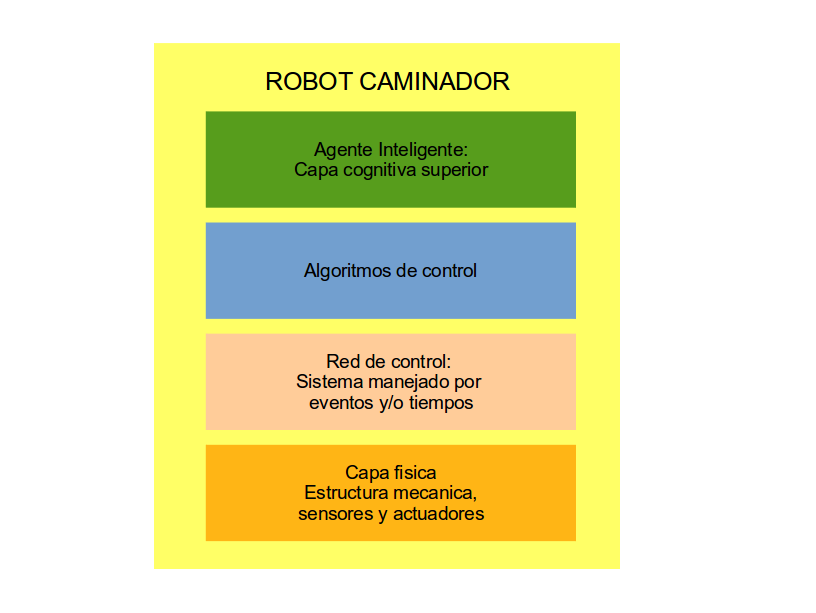
\includegraphics[height=7.0cm]{../images/objGen.png}
    \end{center}
  \end{frame}
  % \begin{frame}
  %   \frametitle{Qu\'e se quiere lograr con esta investigaci\'on?}
  %   \framesubtitle{Framework de investigaci\'on y desarrollo de rob\'otica b\'ipeda}
  %   \begin{center}
  %     \includegraphics[height=1.5cm]{../images/FOBO.png}
  %     \includegraphics[height=1.5cm]{../images/DynamixelRobot.png}
  %     \includegraphics[height=1.5cm]{../images/RABBIT.png}
  %     \includegraphics[height=1.5cm]{../images/DENISE.png}
  %     \includegraphics[height=1.5cm]{../images/TODDLE-MIT.png}
  %     \includegraphics[height=1.5cm]{../images/ASIMO.png}
  %     \includegraphics[height=1.5cm]{../images/DLR-BIPED.png}\\
  %     \includegraphics[height=1.5cm]{../images/IMU-MEMS.png}
  %     \includegraphics[height=1.5cm]{../images/HwArchitectureDesign.png}
  %     \includegraphics[height=1.5cm]{../images/EmbbededLinux.png}
  %     \includegraphics[height=1.5cm]{../images/DynamixelMotor.png}\\
  %     \includegraphics[height=1.5cm]{../images/FlexibleFootDesign.png}
  %     \includegraphics[height=1.5cm]{../images/DarWIN-CAD-FILE.png}
  %     \includegraphics[height=1.5cm]{../images/DarWIN-RENDER.png}
  %     \includegraphics[height=1.5cm]{../images/AirMuscle.png}
  %     \includegraphics[height=1.5cm]{../images/FORCE-TORQUE-Sensor.png}
  %   \end{center}
  % \end{frame}
}
El principal objetivo de esta investigaci\'on se describe de forma global y gr\'afica en la Figura \ref{fig:objGen}, y es enunciado a continuaci\'on:\par
\textbf{OG:} Dise\~nar y construir un \emph{marco de experimentaci\'on}\footnote{compuesto por el dise\~no de una red de sensores-actuadores distribuida y un conjunto de dise\~no de eslanbones y articulaciones modulares para ser frabricados mediante prototipado r\'apido} mediante el cual se pueda implementar\footnote{estudiar, proponer y/o comprobar} las hip\'otesis que solucionen los problemas de locomoci\'on de la rob\'otica subactuada y de caminadores\footnote{que permita la b\'usqueda de estructuras mecatr\'onicas eficientes energ\'eticamente, capaces de lograr la locomoci\'on requerida por las necesidades fundamentales de los robots caminadores}.\par
\begin{figure}[!htb]
  \centering
  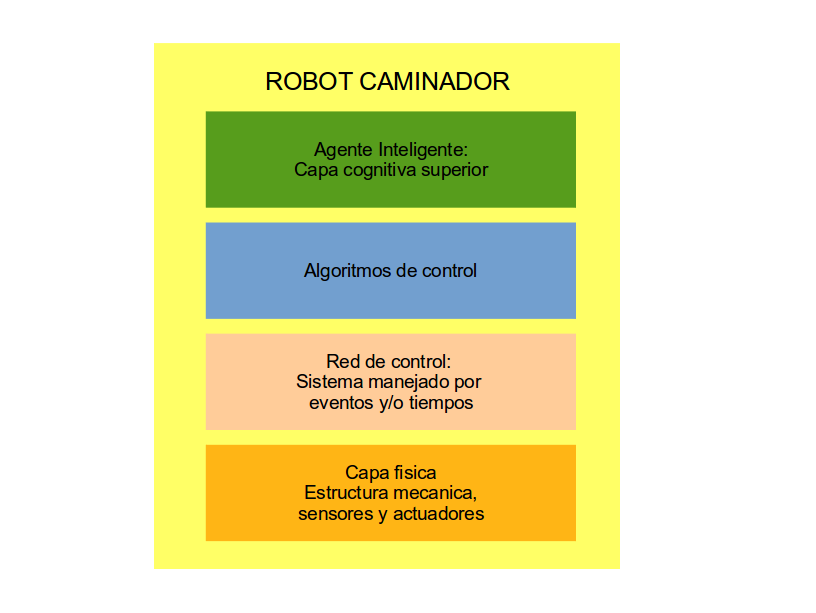
\includegraphics[scale=0.5]{../images/objGen.png}
  \caption{Objetivo General}
  \label{fig:objGen}
\end{figure}

\subsection[Especificos]{Objetivos espec\'ificos}
\label{sec:objesp}
\mode<presentation>{
  \begin{frame}
    \transduration<1->{5}
    \frametitle{Qu\'e se requiere y qu\'e se obtiene para el Obj. Gen?}
    \framesubtitle{Algunos logros requeridos para el objetivo principal}
    \only<1>{
      \begin{center}
        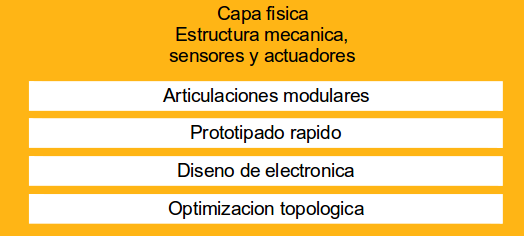
\includegraphics[height=1.0cm]{../images/objCapaFisica.png}
        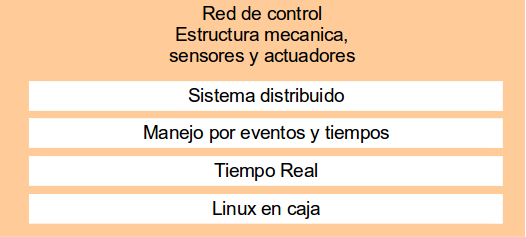
\includegraphics[height=1.0cm]{../images/objCapaRAS.png}
        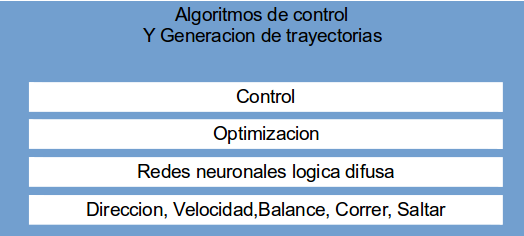
\includegraphics[height=1.0cm]{../images/objCapaControl.png}
        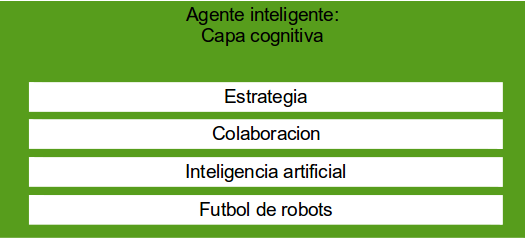
\includegraphics[height=1.0cm]{../images/objCapaCognitiva.png}
      \end{center}
    }
    \only<2>{
      \begin{center}
        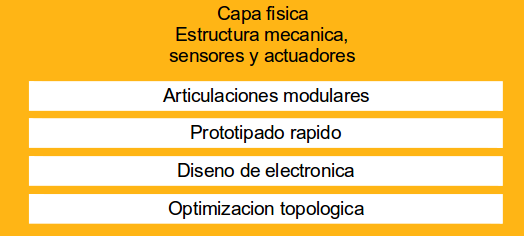
\includegraphics[height=2.5cm]{../images/objCapaFisica.png}
      \end{center}
    }
    \only<3>{
      \begin{center}
        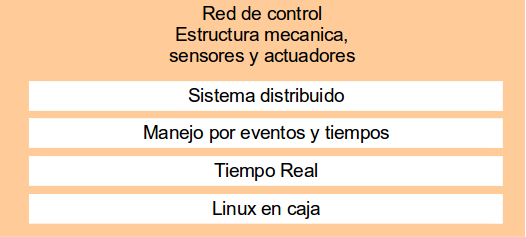
\includegraphics[height=2.5cm]{../images/objCapaRAS.png}
      \end{center}
    }
    \only<4>{
      \begin{center}
        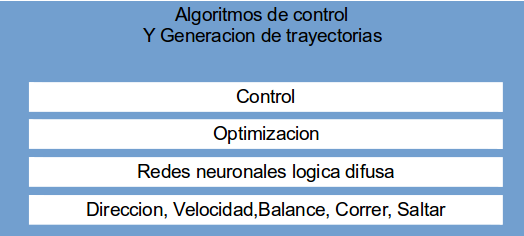
\includegraphics[height=2.5cm]{../images/objCapaControl.png}
      \end{center}
    }
    \only<5>{
      \begin{center}
        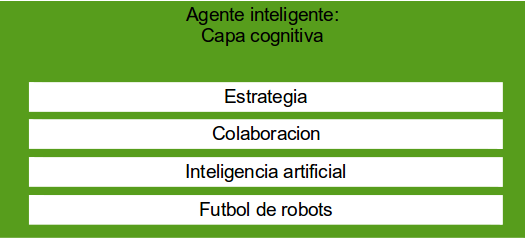
\includegraphics[height=2.5cm]{../images/objCapaCognitiva.png}
      \end{center}
    }
    \begin{enumerate}[<+-|alert@+>][\textbf{OE:} 1.]\scriptsize
    \item Modelar, simular, analizar y sintetizar mecanismos subactuados que optimicen la energ\'ia para la locomoci\'on de caminar, saltar o correr
    \item Dise\~nar y construir una plataforma rob\'otica modular modular y para prototipado, capaz de configurar cadenas cinem\'aticas  controladas y/o monitoreadas bajo el sistema distribuido
    \item Implementar un sistema distribuido de sensores y actuadores que funcione en tiempo-real, bajo el principio de manejo por disparo-de-eventos y/o manejo por disparo-por-tiempos
    \item Dise\~nar, simular e implementar diferentes controles de locomoci\'on inspirados en las nuevas tendencias de investigaci\'on de caminadores sobre plataformas rob\'oticas modulares construidas
    \item Dise\~nar, simular e implementar estrategias y actividades colaborativas usando una red de caminadores.
    \end{enumerate}
  \end{frame}
}
\begin{enumerate}[\textbf{OE:} 1.]
\item Modelar, simular, analizar y sintetizar mecanismos subactuados que optimicen la energ\'ia para la locomoci\'on de caminar, saltar o correr.\par 
\item Dise\~nar y construir una plataforma rob\'otica modular modular y para prototipado (ver Figura \ref{fig:objCapas} Capa Física), capaz de configurar cadenas cinem\'aticas  controladas y/o monitoreadas bajo el sistema distribuido.\par
\item Implementar un sistema distribuido de sensores y actuadores que funcione en tiempo-real  (ver Figura \ref{fig:objCapas} Capa de sensorial y de Actuaci\'on), bajo el principio de manejo por disparo-de-eventos y/o manejo por disparo-por-tiempos\cite{Kimm2012}.\par
\item Dise\~nar, simular e implementar diferentes controles de locomoci\'on (ver Figura \ref{fig:objCapas} Capa de control de locomoci\'on) inspirados en las nuevas tendencias de investigaci\'on de caminadores sobre plataformas rob\'oticas modulares construidas.\par
\item Dise\~nar, simular e implementar estrategias y actividades colaborativas usando una red de caminadores  (ver Figura \ref{fig:objCapas} Capa Cognitiva.).\par
\end{enumerate}
\begin{figure}[!htb]
  \centering
  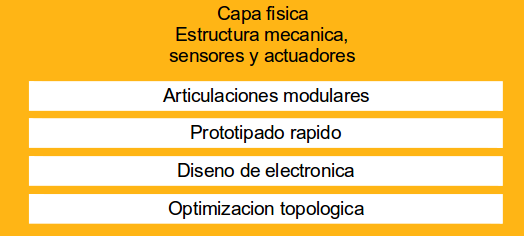
\includegraphics[scale=0.45]{../images/objCapaFisica.png}
  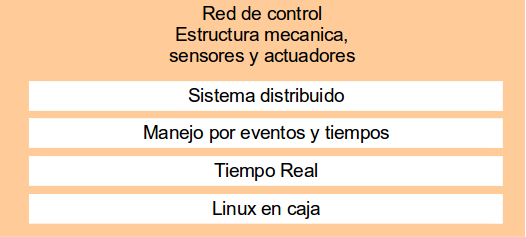
\includegraphics[scale=0.45]{../images/objCapaRAS.png}\\
  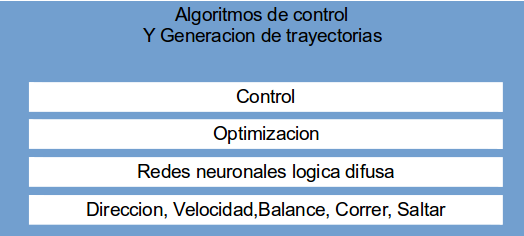
\includegraphics[scale=0.45]{../images/objCapaControl.png}
  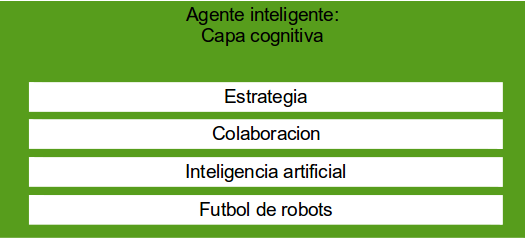
\includegraphics[scale=0.45]{../images/objCapaCognitiva.png}
  \caption{Objetivos Específicos}
  \label{fig:objCapas}
\end{figure}
